\documentclass[tikz,border=5mm]{standalone}

\usepackage[T1]{fontenc}
\usepackage[sfdefault,sb]{plex-sans}
\usepackage{xcolor}
\usepackage{tikz}

\usetikzlibrary{arrows.meta,positioning}

\renewcommand*\familydefault{\sfdefault}

\definecolor{foundationfill}{HTML}{2E64FE}
\definecolor{foundationstroke}{HTML}{153E7E}
\definecolor{corefill}{HTML}{0033CC}
\definecolor{corestroke}{HTML}{001F7A}
\definecolor{advancedfill}{HTML}{000066}
\definecolor{advancedstroke}{HTML}{000033}
\definecolor{edgegray}{HTML}{475569}
\definecolor{crosslinkgray}{HTML}{64748B}
\definecolor{optionalfill}{HTML}{EAF0FF}
\definecolor{optionalstroke}{HTML}{153E7E}

\begin{document}
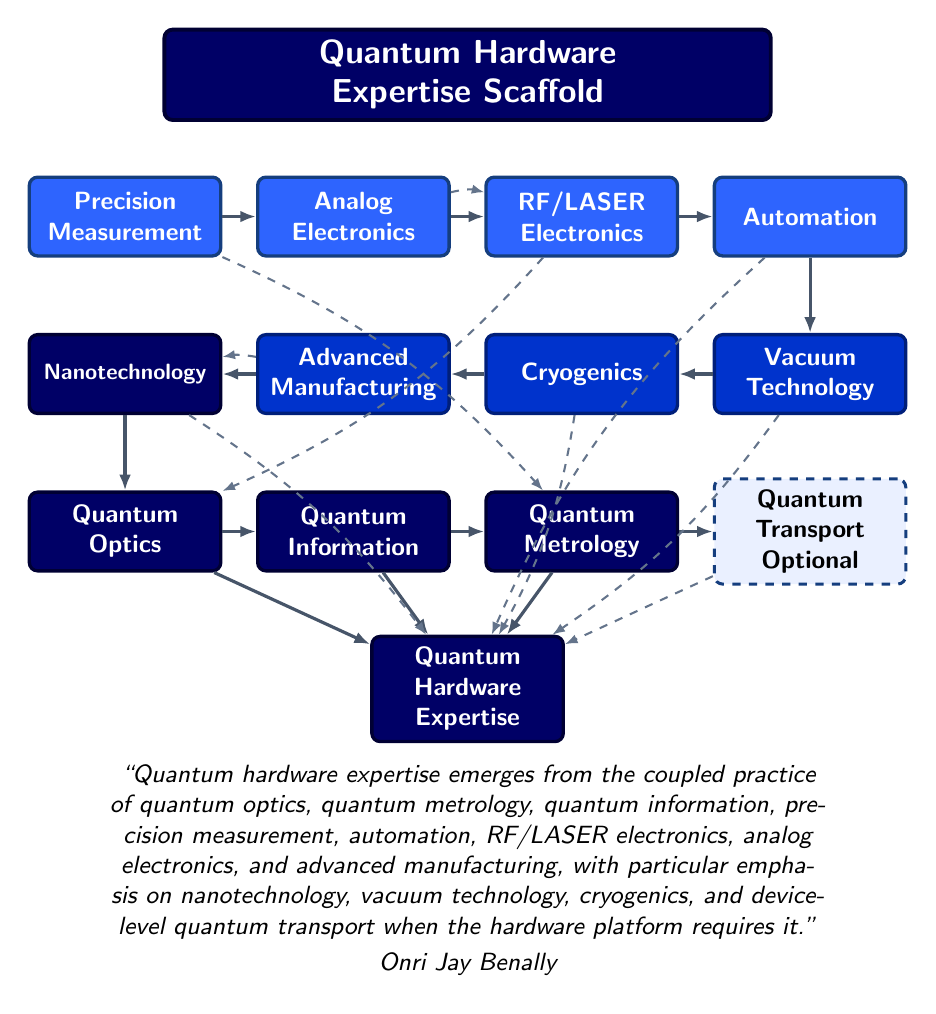
\begin{tikzpicture}[
  x=2.9cm,
  y=-2.0cm,
  every node/.style={
    rectangle,
    rounded corners=3pt,
    align=center,
    inner sep=4pt,
    minimum width=2.35cm,
    minimum height=1.00cm,
    text width=2.15cm,
    font=\small
  },
  scaffold/.style={
    -{Latex[length=2mm]},
    draw=edgegray,
    line width=1.15pt
  },
  crosslink/.style={
    -{Latex[length=1.6mm]},
    draw=crosslinkgray,
    line width=0.75pt,
    dashed
  },
  foundation/.style={
    draw=foundationstroke,
    fill=foundationfill,
    text=white,
    line width=1.2pt,
    font=\bfseries\small
  },
  core/.style={
    draw=corestroke,
    fill=corefill,
    text=white,
    line width=1.2pt,
    font=\bfseries\small
  },
  advanced/.style={
    draw=advancedstroke,
    fill=advancedfill,
    text=white,
    line width=1.2pt,
    font=\bfseries\small
  },
  advancedsmall/.style={
    draw=advancedstroke,
    fill=advancedfill,
    text=white,
    line width=1.2pt,
    font=\bfseries\footnotesize
  },
  optional/.style={
    draw=optionalstroke,
    fill=optionalfill,
    text=black,
    dashed,
    line width=1.1pt,
    font=\bfseries\small
  },
  title/.style={
    draw=advancedstroke,
    fill=advancedfill,
    text=white,
    line width=1.4pt,
    font=\bfseries\large,
    minimum width=7.7cm,
    minimum height=1.0cm,
    text width=7.2cm
  }
]

\node[title] (title) at (1.5,-0.9) {Quantum Hardware Expertise Scaffold};

% Row 1, left to right
\node[foundation] (pm)      at (0,0) {Precision\\Measurement};
\node[foundation] (analog)  at (1,0) {Analog\\Electronics};
\node[foundation] (rf)      at (2,0) {RF/LASER\\Electronics};
\node[foundation] (auto)    at (3,0) {Automation};

% Row 2, right to left
\node[core] (vac)           at (3,1) {Vacuum\\Technology};
\node[core] (cryo)          at (2,1) {Cryogenics};
\node[core] (mfg)           at (1,1) {Advanced\\Manufacturing};
\node[advancedsmall] (nano) at (0,1) {Nanotechnology};

% Row 3, left to right
\node[advanced] (qo)        at (0,2) {Quantum\\Optics};
\node[advanced] (qi)        at (1,2) {Quantum\\Information};
\node[advanced] (qm)        at (2,2) {Quantum\\Metrology};
\node[optional] (qt)        at (3,2) {Quantum\\Transport\\Optional};

% Row 4, capstone
\node[advanced] (qhw)       at (1.5,3) {Quantum\\Hardware\\Expertise};

% Main scaffold path
\draw[scaffold] (pm) -- (analog);
\draw[scaffold] (analog) -- (rf);
\draw[scaffold] (rf) -- (auto);
\draw[scaffold] (auto) -- (vac);

\draw[scaffold] (vac) -- (cryo);
\draw[scaffold] (cryo) -- (mfg);
\draw[scaffold] (mfg) -- (nano);
\draw[scaffold] (nano) -- (qo);

\draw[scaffold] (qo) -- (qi);
\draw[scaffold] (qi) -- (qm);
\draw[scaffold] (qm) -- (qt);

% Final synthesis links
\draw[scaffold] (qo) -- (qhw);
\draw[scaffold] (qi) -- (qhw);
\draw[scaffold] (qm) -- (qhw);
\draw[crosslink] (qt) -- (qhw);

% Supporting cross-links
\draw[crosslink] (pm) to[bend left=12] (qm);
\draw[crosslink] (analog) to[bend left=14] (rf);
\draw[crosslink] (rf) to[bend left=12] (qo);
\draw[crosslink] (auto) to[bend right=12] (qhw);

\draw[crosslink] (vac) to[bend left=10] (qhw);
\draw[crosslink] (cryo) to[bend left=10] (qhw);
\draw[crosslink] (mfg) to[bend right=10] (nano);
\draw[crosslink] (nano) to[bend left=10] (qhw);

% Optional quote attribution
\node[
  align=center,
  font=\small\itshape,
  text width=10.4cm
] at (1.5,4.15)
{``Quantum hardware expertise emerges from the coupled practice of quantum optics, quantum metrology, quantum information, precision measurement, automation, RF/LASER electronics, analog electronics, and advanced manufacturing, with particular emphasis on nanotechnology, vacuum technology, cryogenics, and device-level quantum transport when the hardware platform requires it.''\\[2pt]
Onri Jay Benally};

\end{tikzpicture}
\end{document}
